%
% polynom.tex
%
% (c) 2020 Prof Dr Andreas Müller, Hochschule Rapeprswil
%
\section{Interpolationspolynom
\label{buch:section:interpolationspolynom}}
\rhead{Lagrange-Interpolationspolynome}
In diesem Abschnitt wird das folgende Problem gelöst.
\begin{aufgabe}[Interplations-Polynom]
Gegeben Stützstellen
\[
a=x_0<x_1<x_2<\dots < x_{n-1}<x_n=b
\]
und Funktionswerte $f_i, 0\le i\le n$, finde ein Polynome $l(x)$
mit der Eigenschaft $l(x_i)=f_i$ für alle $i=0,1,\dots n$.
\end{aufgabe}
Gegeben sind also $n+1$ Bedingungen, die das Polynom erfüllen muss.
Abgesehen von trivialen Fällen wie dem Null-Polynom, muss ein Polynom
im Allgemeinen mindestens den Grad $n$ haben, damit alle 
Bedingungen durch geeignete Wahl der $n+1$ Koeffizienten erfüllt werden können.
Man könnte das Polynom nämlich in der Form
\[
l(x)
=
a_nx^n + a_{n-1}x^{n-1}+\dots+a_1x+a_0
\]
ansetzen und die Stützstellen einsetzen.
Lösung des Gleichungssystem
\begin{equation}
\begin{linsys}{5}
a_Nx_0^N &+& a_{N-1}x_0^{N-1} &+& \dots &+& a_1x_0 &+& a_0x_0 &=& f_0 \\[5pt]
a_Nx_1^N &+& a_{N-1}x_1^{N-1} &+& \dots &+& a_1x_1 &+& a_0x_1 &=& f_1 \\[5pt]
\vdots   & &    \vdots        & & \ddots& & \vdots & & \vdots & & \vdots\\[5pt]
a_Nx_n^N &+& a_{N-1}x_n^{N-1} &+& \dots &+& a_1x_n &+& a_0x_n &=& f_n 
\end{linsys}
\end{equation}
liefert dann die gesuchten Koeffizienten.
Dieser Weg ist allerdings sehr aufwendig, die Lösung eines linearen
Gleichungssystems mit dem Gauss-Algorithmus benötigt $O(n^3)$ Operationen.
Die sehr spezielle Struktur des Gleichungssystems sollte ermöglichen,
das Polynom $l(x)$ auf direkterem Weg zu ermitteln.

%
% Interpolationspolynom bestimmen
%
\subsection{Bestimmung des Interpolationspolynoms
\label{buch:section:interpolation:bestimmung}}
Das allgemeine Interpolationsproblem kann leicht gelöst werden, wenn
das folgende spezielle Interpolationsproblem gelöst ist.

\begin{aufgabe}[Spezielle Interpolationspolynome]
Gegeben die Stützstellen
\[
a=x_0<x_1<x_2<\dots <x_{n-1}<x_n=b,
\]
finde Polynome $l_j$ vom Grad $n$ derart, dass
\[
l_j(x_i) = \delta_{ij}=\begin{cases}
1&\qquad i=j\\
0&\qquad\text{sonst.}
\end{cases}
\]
\end{aufgabe}

Jedes der Interpolationspolynome $l_j$ hat Grad $n$, also hat auch eine
beliebige Linearkombination den Grad höchstens $n$.
Die Linearkombination
\[
l(x) = \sum_{j=0}^n f_j l_j(x)
\]
ist das gesuchte Interpolationspolynom, wie Einsetzen von $x_i$ in
\[
l(x_i)
=
\sum_{j=0}^n f_jl_j(x_i)
=
\sum_{j=0}^n f_j\delta_{ij}
=
f_i
\]
bestätigt.

\begin{beispiel}
Ein besonders einfacher Fall ist $n=1$.
Gesucht ist eine lineare Funktion $l(x)=a_1x+a_0$ derart, dass
$l(x_0)=f_0$ und $l(x_1)=f_1$.
Polynome $l_0$ und $l_1$ können leicht angegeben werden:
\[
l_0(x) = \frac{x_1-x}{x_1-x_0}
\qquad\text{und}\qquad
l_1(x) = \frac{x-x_0}{x_1-x_0}
\]
haben die die geforderten Eigenschaften.
Die gesuchte Interplationsfunktion ist daher
\[
l(x)
=
\frac{x_1-x}{x_1-x_0}f_0 + \frac{x-x_0}{x_1-x_0} f_1
=
x \frac{f_1-f_0}{x_1-x_0}   + \frac{x_1f_0-x_0f_1}{x_1-x_0}.
\]
Der Koeffizient von $x$ ist wie erwartet die Steigung der Geraden durch
die Punkte $(x_0,f_0)$ und $(x_1,f_1)$.
\end{beispiel}

Ein Polynom vom Grad $n+1$, welches in {\em allen} Stützstellen verschwindet,
ist leicht zu finden, es ist 
\[
(x-x_0)(x-x_1)(x-x_2)\dots (x-x_{n-1})(x-x_n).
\]
Ein Polynom, welches nur an der Stützstelle $x_j$ {\em nicht} verschwindet,
ensteht, indem man den Faktor $(x-x_j)$ weglässt, es hat den Grad $n$.
Wir führen dafür die Notation
\[
(x-x_0)(x-x_1)(x-x_2)\dots \widehat{(x-x_j)}\dots (x-x_{n-1}(x-x_n),
\]
der Hut bedeutet, dass dieser Faktor weggelassen werden soll.
Allerdings hat dieses Polynom nicht den geforderten Wert $1$, man muss es
also noch mit einer geeigneten Konstante multiplizieren.
Das gesuchte Polynom $l_j(x)$ hat daher die Form
\[
l_j(x)
=
c_j(x-x_0)(x-x_1)(x-x_2)\dots \widehat{(x-x_j)}\dots (x-x_{n-1}(x-x_n).
\]
Einesetzen von $x_j$ ergibt
\[
l_j(x_j) = 1 = 
c_j(x_j-x_0)(x_j-x_1)(x_j-x_2)\dots \widehat{(x_j-x_j)}\dots(x_j-x_{n-1}(x_j-x_n),
\]
die Konstante $c_j$ ist daher
\[
c_j = \prod_{i=0\atop i\ne j}^n \frac{1}{x_j-x_i}.
\]

\begin{beispiel}
Man finde ein Polynome, welches $l(0)=l(1)=0$ und $l(\frac12)=1$
erfüllt.
Wegen $f_0=f_2=0$ ist nur das Polynome $l_1$ zu ermitteln, es ist
\[
l(x) = l_1(x)
=
\frac{(x-x_0)(x-x_2)}{(x_1-x_0)(x_1-x_2)}
=
\frac{x(x-1)}{\frac12(\frac12-1)}
=
\frac14x(1-x).
\qedhere
\]
\end{beispiel}

%
% Fehler des Interpolationspolynoms
%
\subsection{Fehler von Approximationspolynomen
\label{buch:section:interpolation:fehler}}
Getreu der Maxime, dass wir zu jeder numerischen Lösungsformel auch
Informationen über die zu erwartenden Fehler brauchen, entwickeln
wir in diesem Abschnitt die Theorie des Fehlers der Approximationspolynome.
Wir müssen zu diesem Zweck einen kleinen Ausflug in die Analysis unternehmen
in einen Bereich, der im Unterricht manchmal etwas zu kurz kommt.

Wenn die Ableitung einer Funktion in einem Interval klein ist,
dann werden auch die Funktionswerte im Inneren dieses Intervals
nicht gross von den Werten am Rand abweichen können.
Eine grosse Abweichung würde ja automatisch eine Steigung einer Sekanten
und damit auch eine grosse Steigung einer Tangenten zur Folge haben.
Dies ist die Idee, die den nachfolgend entwickelten Fehlerabschätzungen
zu Grunde liegt.

\subsubsection{Der Zwischenwertsatz}
Der Ausgangspunkt aller nachfolgenden Überlegungen ist die intuitiv
anschauliche Tatsache, dass eine stetige Funktion keine Sprünge macht.

\begin{satz}
Eine auf dem Intervall $[a,b]$ stetige Funktion nimmt jeden Wert im
Interval $[f(a),f(b)]$ an.
Anders ausgedrückt, für jedes $y$ zwischen $f(a)$ und $f(b)$ gibt es ein 
$x$ zwischen $a$ und $b$ derart, dass $y=f(x)$.
\end{satz}

Dieser Satz war natürlich bereits die Grundlage des Verfahrens der
Interval-Halbierung, mit welchem wir in
Abschnitt~\ref{buch:subsection:intervallhalbierung}
Gleichungen gelöst haben.
Wenn die Funktion an den Intervallenden verschiedene Vorzeichen hat,
dann muss es eine Nullstelle im Inneren des Intervalls geben.
Die Intervallhalbierung hat in jedem Schritt ein neues Intervall
konstruiert, das die Nullstelle enthielt.

\subsubsection{Der Satz von Rolle}
\begin{figure}
\centering
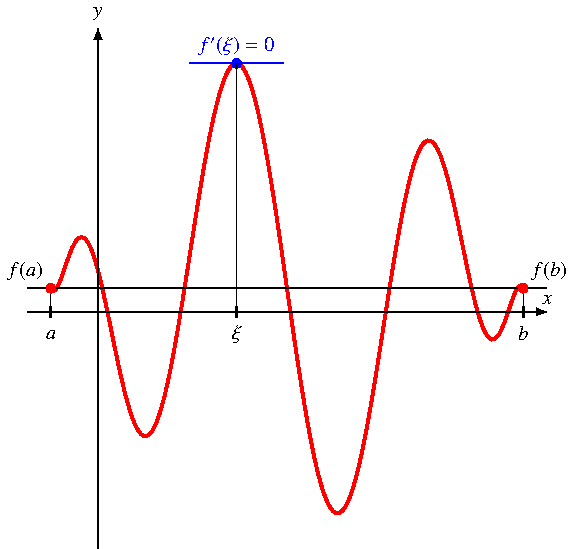
\includegraphics{chapters/30-interpolation/figures/rolle.pdf}
\caption{Satz von Rolle: eine nicht konstante differenzierbare Funktion,
die an den Enden eines Intervals den gleichen Funktionswert hat, hat im 
Inneren des Intervals eine Stelle $\xi$ mit Ableitung $0$.
\label{buch:figure:rolle}}
\end{figure}
Der Satz von Rolle erweitert den Zwischenwertsatz auf die Ableitung einer
differenzierbaren Funktion an (Abbildung~\ref{buch:figure:rolle}).

\begin{satz}[Rolle]
\label{buch:satz:rolle}
Sei $f$ eine auf dem Interval $[a,b]$ nicht konstante,
stetig differenzierbare Funktion
mit $f(a)=f(b)$, dann gibt es einen Punkt $\xi\in(a,b)]$ im Inneren
des derart, dass $f'(\xi)=0$.
\end{satz}

Der Satz von Rolle ist eine selbstverständlichkeit, wenn die Ableitung
$f'(x)$ stetig ist, doch dies wird nicht vorausgesetzt, es wird nur
verlangt, dass die Ableitung existiert.
Ausserdem macht der Satz eine Aussage darüber, dass die Zwischenstelle
$\xi$ im Inneren des Intervals sei.

\begin{proof}[Beweis]
Eine stetige Funktion hat auf dem kompakten Interval $[a,b]$ mindestens
ein Maximum und ein Minimum.
Da die Funktion nicht konstant ist, ist das Maximum oder das Minimum
von $f(a)$ verschieden.
Wir nehmen an $\xi\in[a,b]$ sei ein Maximum mit dieser Eigenschaft,
das Argument für das Minimum ist völlig analog.
Wegen $f(\xi)>f(a)$ ist $\xi$ ein Punkt im Inneren des Intervals,
also $\xi\in(a,b)$.

Wegen $f(\xi) \ge f(x)\forall x\in[a,b]$
folgt dann
\begin{align*}
f'(\xi) &= \lim_{h\to 0+}  \frac{f(\xi+h)-f(\xi)}{h} \le 0
\\
f'(\xi) &= \lim_{h\to 0-}  \frac{f(\xi+h)-f(\xi)}{h} \ge 0.
\end{align*}
Da $f$ differenzierbar ist, müssen diese beiden Grenzwerte übereinstimmen,
also ist $f'(\xi)=0$.
\end{proof}


\subsubsection{Nullstellen und der Satz von Rolle}
\begin{figure}
\centering
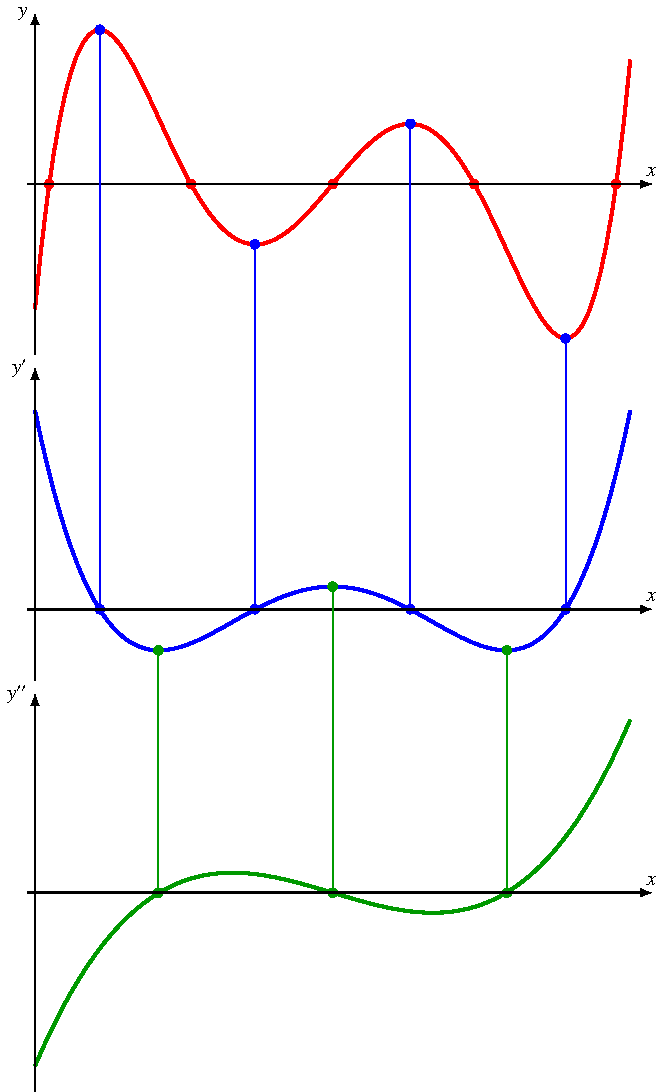
\includegraphics{chapters/30-interpolation/figures/nullstellen.pdf}
\caption{Schachtelung der Nullstellen von $f(x)$, $f'(x)$ und $f''(x)$.
Der Satz von Rolle~\ref{buch:satz:rolle} impliziert, dass sich zwischen zwei
Nullstellen von $f$ immer eine Nullstelle von $f'$ befindet, und
ebenso zwischen zwei Nullstellen von $f'$ eine von $f''$.
\label{buch:figure:nullstellen}}
\end{figure}

\begin{satz}
\label{buch:satz:nullstellen}
Ist $f$ eine differenzierbare Funktion auf dem Intervall $[a,b]$
mit Nullstellen 
\[
a=x_0 < x_1 < x_2 < \dots < x_{n-1} < x_n = b,
\]
die auf keinem Teilintervall $[x_i,x_{i+1}]$ konstant ist,
dann hat $f'$ im Inneren jedes Teilintervalls $[x_i, x_{i+1}]$
eine Nullstelle.
\end{satz}

Das Polynom 
\[
l(x) = (x-x_0)(x-x_1)\dots (x-x_{n-1})(x-x_n),
\]
welches für die Konstruktion des Interpolationspolynoms verwendet
wurde, hat genau die Nullstellen $x_0,x_1,\dots,x_{n-1},x_n$.
Nach dem Satz~\ref{buch:satz:nullstellen} muss es zwischen je
zwei aufeinanderfolgenden Nullstellen von $l$ eine Nullstelle der
Ableitung geben. 
Diese Situation ist in Abbildung~\ref{buch:figure:nullstellen}
für den Fall $l(x)=(x+2)(x+1)x(x-1)(x-2)$ dargestellt.

Die höheren Ableitungen $f^{(k)}$ haben ihre Nullstellen
natürlich auch wieder zwischen den Nullstellen der Ableitung $f^{(k-1)}$.
Die $n$-te Ableitung ist konstant und hat keine Nullstellen.

\begin{figure}
\centering
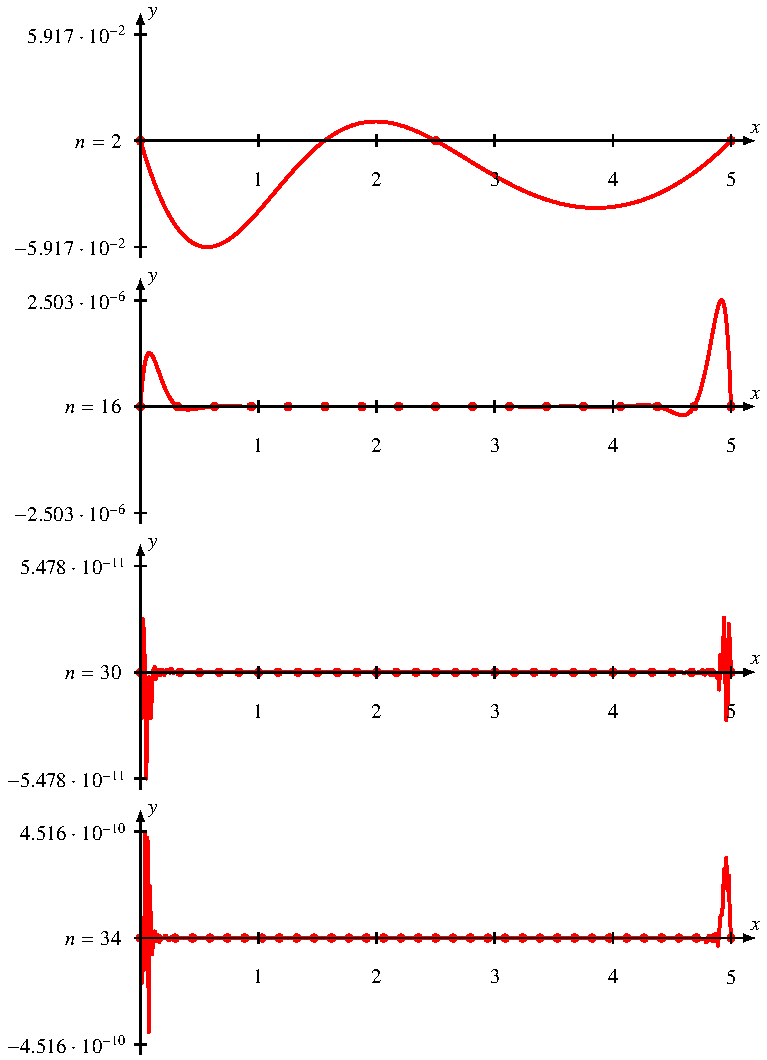
\includegraphics{chapters/30-interpolation/figures/norm.pdf}
\caption{Fehler des Lagrange-Interpolationspolynoms für die Funktion
$f(x)=e^{-x^2/2}/\sqrt{2\pi}$.
Der Fehler nimmt mit der Anzahl der Stützstellen bis $n=30$ ab, danach
wird die Berechnung instabil und der Fehler nimmt wieder zu.
\label{buch:figure:lagrangefehler}}
\end{figure}

\subsubsection{Der Mittelwertsatz der Differentialrechnung}

\subsubsection{Taylorreihe mit Restformel}

\subsubsection{Fehler des Lagrange-Interpolationspolynoms}
Der folgende satz gibt vollständige Auskunft über den Fehler des
Interpolationspolynoms.

\begin{satz}
\label{buch:satz:lagrangefehler}
Sei $p$ ein Polynom vom Grad $n$, welches mit der $n+1$-mal differenzierbaren
Funktion $f$ an den $n+1$ Stellen
\[
a = x_0 < x_1 < x_2 < \dots  < x_{n-1} < x_n=b
\]
übereinstimmt.
Dann gibt es für jedes $x\in[a,b]$ ein $\xi_x\in [a,b]$ mit
\begin{equation}
f(x) - p(x) = \frac{f^{(n+1)}(\xi_x)}{(n+1)!} l(x)
\label{buch:equation:polyfehler}
\end{equation}
\end{satz}

\begin{proof}[Beweis]
An den Stützstellen $x_i$ ist $f(x_i)-p(x_i)=0$ und $l(x_i)=0$, die
Gleichung~\eqref{buch:equation:polyfehler} ist also trivialerweise
erfüllt.

Sei jetzt also $x\in[a,b]$ verschieden von allen $x_i$.
Da $l(x)\ne 0$ ist, gibt es eine Zahl $c$ derart, dass
\begin{equation}
f(x)-p(x)=cl(x)
\qquad\Leftrightarrow\qquad
f(x)-p(x)-cl(x)=0.
\label{buch:equation:polyfehler1}
\end{equation}
Die Funktion $g(x)=f(x)-p(x)-cl(x)$ verschwindet in allen Stützstellen $x_i$
und zusätzlich auch noch im Punkt $x$, sie hat also $n+1$ Nullstellen.

Nach dem Nullstellen-Schachtelungssatz~\ref{buch:satz:nullstellen}
hat die $n+1$ Ableitung von $g$ eine Nullstelle im Intervall.
Es gibt also eine Zahl $\xi_x\in[a,b]$ mit $g^{(n+1)}(\xi_x)=0$.

Da $p$ Grad $n$ hat, ist die $n+1$-te Ableitung $0$.
Das Polynom $l(x)$ hat die Form
\[
l(x) = x^{n+1} -(x_0+x_1+\dots+x_{n-1}+x_n)x^{n-1} + \dots + (-1)^{n+1}x_0x_1\dots x_{n-1}x_n,
\]
seine $n+1$-Ableitung ist die Konstanten $(n+1)!$.

Die Folgerung $g^{(n+1)}(\xi_x)=0$ wird damit zu
\[
0 = f^{(n+1)}(\xi_x) -c (n+1)!
\qquad\Rightarrow\quad
c=\frac{f^{(n+1)}(\xi_x)}{(n+1)!}.
\]
Einsetzen in \eqref{buch:equation:polyfehler1} ergibt
\[
f(x)-p(x) = cl(x)=\frac{f^{(n+1)}(\xi_x)}{(n+1)!} l(x),
\]
wie behauptet.
\end{proof}

Dieser Satz erlaubt den Fehler eines Interpolationspolynoms abzuschätzen,
wenn die $n+1$-te Ableitung der Funktion $f$ bekannt ist.
Wir bezeichnen mit
\[
\|g\| = \sup_{a\le x\le b} |g(x)|
\]
die {\em Supremun-Norm} der Funktion $g$ im Intervall $[a,b]$.
\index{Supremum-Norm}

\begin{korollar}
\label{buch:korollar:interpolationsfehler}
Ist $p$ ein Interpolationspolynom vom Grad $n$, welches mit der Funktion
$f$ in den Stellen $a=x_0<x_1<\dots <x_{n+1}<x_n=b$ übereinstimmt, dann
ist 
\[
|f(x)-p(x)| \le \frac{\|f^{(n+1)}\|}{(n+1)!} |l(x)|.
\]
\end{korollar}

\begin{beispiel}
\begin{figure}
\centering
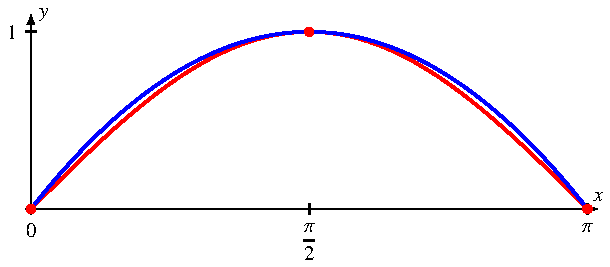
\includegraphics{chapters/30-interpolation/figures/sin.pdf}
\caption{Interpolation der Funktion $f(x)=\sin x$ mit nur drei 
Stützstellen $x_0=0$, $x_1=\frac{\pi}2$ und $x_2=\pi$.
Der Fehler ist deutlich kleiner als die Abschätzung mit
Satz~\ref{buch:satz:lagrangefehler} erwarten lässt.
\label{buch:figure:sin}}
\end{figure}
Die Funktion $f(x)=\sin x$ soll mit den Stützstellen $x_0=0$, $x_1=\frac{\pi}2$
und $x_2=\pi$ interpoliert werden.
Das Interpolationspolynom ist ein quadratisches Polynom mit Nullstellen
$x_0$ und $x_2$, der Funktionswert bei $x_1$ muss $1$ sein.
Man kann sich davon überzeugen, dass das Polynom
\[
p(x) = \frac{4}{\pi^2} x(\pi -x )
\]
diese Eigenschaft hat.
Wie gross ist der Fehler dieses Interpolationspolynoms?

Die dritten Ableitungen der Funktion $f(x)=\sin x$ sind, bekannt, es ist
$f^{(3)}(x)=-\cos x$.
Der Betrag von $f^{(3)}(x)$ wird also nie grösser als $1$.
Es folgt, dass
\[
|f(x)-p(x)| \le \frac{1}{3!} l(x)
=
\frac16 |x(x-{\textstyle\frac{\pi}2})(x-\pi)|
\]
Die Ableitung des Polynoms auf der rechten Seite hat Nullstellen bei
$\frac{\pi}2 \pm \frac{\pi}{2\sqrt{3}}$,
durch Einsetzen erhält man den maximalen Wert
\[
\|f^{(3)}\|
=
\frac{\pi^3}{12\sqrt{3}}\simeq 1.49179.
\]
Wir schliessen, dass das Interpolationspolynom niemals um mehr als $0.24863$
vom Funktionswert abweichen kann.
\end{beispiel}

%
% Tschebyscheff Interpolation
%
\subsection{Wahl der Stützstellen und Tschebyscheff-Interpolationspolynom
\label{buch:section:interpolation:tschebyscheff}}
Das Korllar~\ref{buch:korollar:interpolationsfehler} besagt, dass der
Fehler des Interplationspolynom durch den Betrag von $l(x)$ begrenzt
ist.



\begin{figure}
\centering
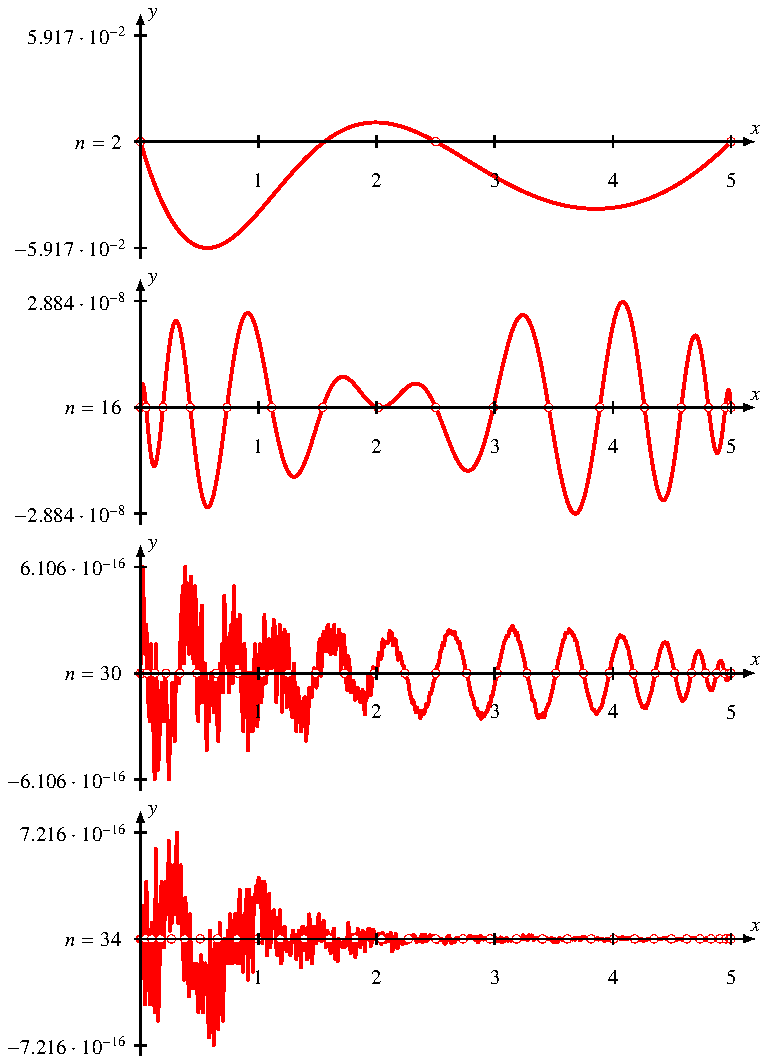
\includegraphics{chapters/30-interpolation/figures/tscheb.pdf}
\caption{Fehler des Interpolationspolynomes für die Funktion
$f(x)=e^{-x^2/2}/\sqrt{2\pi}$ mit Stützstellen nach Tschebyscheff.
Der Fehler bleibt über das ganze Intervall gleichmässig.
Für eine grosse Zahl von Stützstellen erreicht die Interpolation die
Maschienengenauigkeit.
\label{buch:figure:tschebyschefffehler}}
\end{figure}
